\chapter{Survival Prognosis Replication: Results and Discussion}
\label{ch:study2_results}

This chapter presents and discusses the results of Study~II.
Section~\ref{sec:s2r_cohort} describes the final cohort and class distribution.
Sections~\ref{sec:s2r_cv} and~\ref{sec:s2r_test} report cross-validation and held-out test performance.
Section~\ref{sec:s2r_decoupling} analyses the AUC--sensitivity decoupling identified in the MLP model.
Section~\ref{sec:s2r_threshold} presents the decision threshold analysis.
Section~\ref{sec:s2r_bagging} presents the BalancedBagging replication and statistical tests.
Section~\ref{sec:s2r_comparison} compares this study with Papaiz et al.
Section~\ref{sec:s2r_shap} discusses SHAP-based model interpretation.
Sections~\ref{sec:s2r_limitations} and~\ref{sec:s2r_summary} cover limitations and a synthesis of the main findings.

% ============================================================
\section{Cohort and Class Distribution}
\label{sec:s2r_cohort}
% ============================================================

After applying all eligibility filters (censored patients, missing FVC/BMI, ambiguous site of onset), the final cohort comprises 1,502 patients: 174 Short Survivors (11.6\%) and 1,328 Standard Survival patients (88.4\%).
The train/test partition yields 1,201 training patients (139 Short Survivors, 1,062 Standard Survival) and 301 test patients (35 Short Survivors, 266 Standard Survival).

This imbalance ratio of 7.6:1 is substantially more severe than the 2.3:1 ratio of Study~I.
A classifier that labels all patients as Standard Survival achieves 88.4\% accuracy while detecting zero Short Survivors.
ROC-AUC alone does not distinguish such a degenerate model from a clinically useful one, motivating the focus on sensitivity and threshold-aware evaluation throughout this chapter.

% ============================================================
\section{Cross-Validation Performance}
\label{sec:s2r_cv}
% ============================================================

Table~\ref{tab:s2_cv} shows, for each classifier, the highest-AUC configuration found across 70 Optuna-optimised combinations, averaged over 15 cross-validation folds.

\begin{table}[ht!]
  \centering
  \caption[Best cross-validation results per classifier (Study II)]{Best cross-validation results per classifier (Optuna, 70 combinations, 15-fold repeated CV). Sensitivity and specificity refer to the Short Survivor (minority) class. G-Mean $= \sqrt{\text{Sensitivity} \times \text{Specificity}}$.}
  \label{tab:s2_cv}
  \resizebox{\linewidth}{!}{%
  \begin{tabular}{llcccc}
    \toprule
    \textbf{Classifier} & \textbf{Best Technique} & \textbf{AUC}
      & \textbf{Sensitivity} & \textbf{Specificity} & \textbf{G-Mean} \\
    \midrule
    MLP           & None       & 0.915 & 0.427 & 0.969 & 0.641 \\
    LightGBM      & ROS        & 0.914 & 0.780 & 0.864 & 0.819 \\
    SVM           & SMOTEENN   & 0.911 & 0.904 & 0.784 & 0.842 \\
    Random Forest & None       & 0.906 & 0.276 & 0.983 & 0.517 \\
    Naïve Bayes   & None       & 0.891 & 0.727 & 0.867 & 0.793 \\
    KNN           & RUS        & 0.880 & 0.767 & 0.831 & 0.797 \\
    Decision Tree & TomekLinks & 0.861 & 0.413 & 0.948 & 0.621 \\
    \bottomrule
  \end{tabular}%
  }
\end{table}

The MLP achieves the highest cross-validation AUC (0.915) but at the cost of low minority-class sensitivity (0.427).
The Optuna configuration behind this result carries a comparatively strong L2 penalty ($\alpha = 0.061$), roughly five times larger than values found for the same architecture under any resampling strategy.
This may indicate that regularisation suppresses the model's tendency to assign uniformly high scores to Standard Survival patients, improving probability ranking (and therefore AUC) without pushing minority-class scores above the 0.5 decision boundary.

LightGBM with Random Oversampling sits one AUC point behind (0.914) but delivers sensitivity of 0.780 and G-Mean of 0.819.
Three classifiers---MLP, Random Forest, and Naïve Bayes---reach their best AUC with no imbalance correction at all; for MLP and Random Forest, that high AUC coexists with poor sensitivity.
The held-out test makes this gap impossible to ignore.

% ============================================================
\section{Held-Out Test Set Evaluation}
\label{sec:s2r_test}
% ============================================================

After model selection was finalised on the training set, each classifier was retrained on the full training partition and evaluated on the sealed test set (35 Short Survivors, 266 Standard Survival patients).
Results appear in Table~\ref{tab:s2_test}.

\begin{table}[ht!]
  \centering
  \caption[Held-out test performance with 95\% bootstrap CI]{Held-out test set performance for each classifier under its best cross-validation configuration. Each cell shows the point estimate with the bootstrap 95\% percentile confidence interval in parentheses (2,000 resamples; no bootstrap sample contained zero Short Survivors). Bold indicates the best point estimate per metric. With 35 Short Survivors, one patient $= 2.86$\,pp; the sensitivity CIs of LightGBM+ROS and SVM+SMOTEENN overlap, indicating the one-patient difference is not statistically distinguishable given the 35-patient minority class.}
  \label{tab:s2_test}
  \resizebox{\linewidth}{!}{%
  \begin{tabular}{llccccc}
    \toprule
    \textbf{Classifier} & \textbf{Technique} & \textbf{AUC}
      & \textbf{Bal.\ Acc.} & \textbf{Sensitivity} & \textbf{Specificity}
      & \textbf{G-Mean} \\
    \midrule
    LightGBM
      & ROS
      & \textbf{0.923} {\small(0.868--0.966)}
      & \textbf{0.844} {\small(0.774--0.903)}
      & 0.857 {\small(0.724--0.967)}
      & 0.831 {\small(0.784--0.876)}
      & \textbf{0.844} {\small(0.772--0.902)} \\
    Random Forest
      & None
      & 0.919 {\small(0.868--0.958)}
      & 0.623 {\small(0.551--0.700)}
      & 0.257 {\small(0.114--0.412)}
      & 0.989 {\small(0.974--1.000)}
      & 0.504 {\small(0.337--0.638)} \\
    MLP
      & None
      & 0.918 {\small(0.874--0.955)}
      & 0.514 {\small(0.500--0.550)}
      & 0.029 {\small(0.000--0.100)}
      & \textbf{1.000} {\small(1.000--1.000)}
      & 0.169 {\small(0.000--0.316)} \\
    SVM
      & SMOTEENN
      & 0.908 {\small(0.863--0.946)}
      & 0.826 {\small(0.759--0.880)}
      & \textbf{0.886} {\small(0.765--0.975)}
      & 0.767 {\small(0.714--0.821)}
      & 0.824 {\small(0.758--0.875)} \\
    Naïve Bayes
      & None
      & 0.889 {\small(0.834--0.937)}
      & 0.774 {\small(0.694--0.847)}
      & 0.714 {\small(0.556--0.853)}
      & 0.835 {\small(0.789--0.881)}
      & 0.772 {\small(0.682--0.847)} \\
    KNN
      & RUS
      & 0.886 {\small(0.834--0.933)}
      & 0.812 {\small(0.738--0.879)}
      & 0.800 {\small(0.655--0.925)}
      & 0.823 {\small(0.779--0.870)}
      & 0.812 {\small(0.735--0.878)} \\
    Decision Tree
      & TomekLinks
      & 0.874 {\small(0.805--0.931)}
      & 0.628 {\small(0.555--0.706)}
      & 0.286 {\small(0.136--0.440)}
      & 0.970 {\small(0.948--0.989)}
      & 0.526 {\small(0.364--0.654)} \\
    \bottomrule
  \end{tabular}%
  }
\end{table}

LightGBM with Random Oversampling identified 30 of 35 Short Survivors (sensitivity 0.857, 95\%\,CI [0.724,\,0.967]; specificity 0.831; AUC 0.923).
SVM with SMOTEENN caught 31 of 35 (sensitivity 0.886, 95\%\,CI [0.765,\,0.975]), but at lower specificity (0.767) and AUC (0.909).
The sensitivity confidence intervals of these two models overlap substantially: the one-patient difference is not statistically distinguishable given the 35-patient minority class.
Both models serve different use cases---SVM+SMOTEENN when missing a Short Survivor is the worst outcome; LightGBM+ROS when overall balance across all metrics matters.

Figures~\ref{fig:s2_cvtest} and~\ref{fig:s2_decoupling} show the AUC comparison across all seven classifiers.

\begin{figure}[ht!]
  \centering
  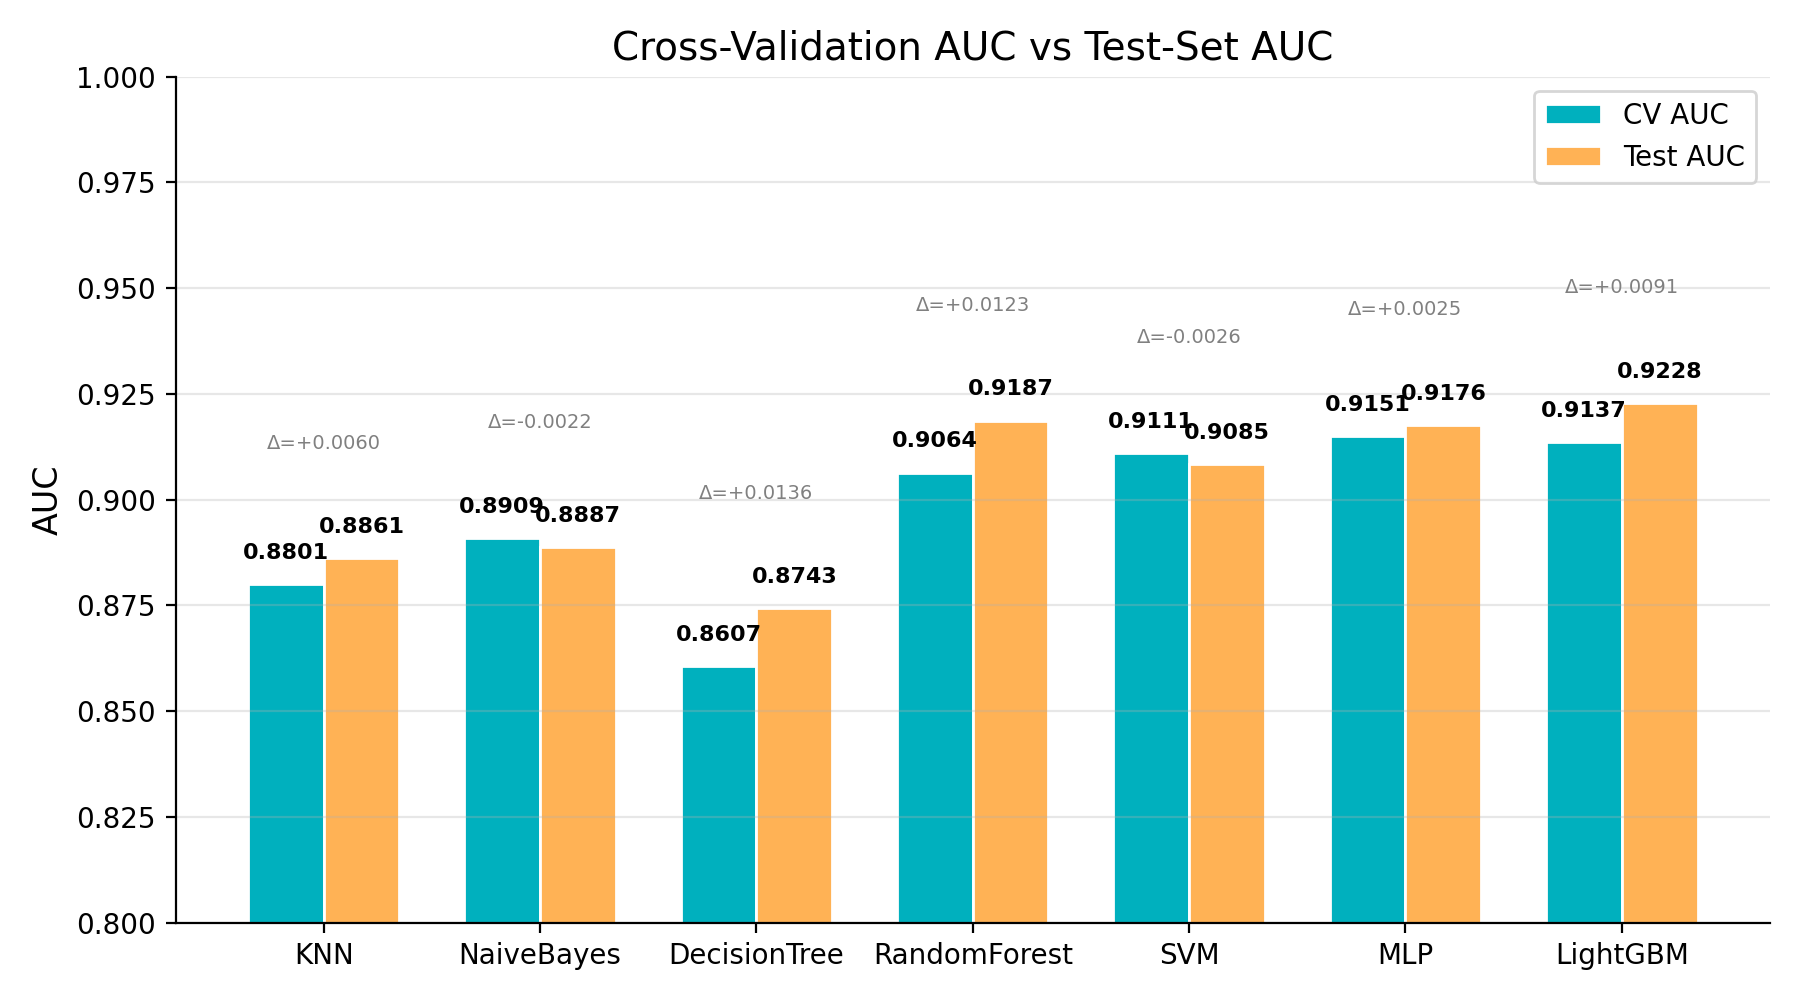
\includegraphics[width=0.95\linewidth]{images/figures/step6_cv_vs_test.png}
  \caption[CV AUC vs.\ test AUC by classifier]{Cross-validation AUC versus held-out test AUC for all seven classifiers under their best configurations. The MLP ranks first in CV AUC (0.915) yet achieves near-chance sensitivity on the test set (0.029), illustrating the AUC--sensitivity decoupling under severe class imbalance.}
  \label{fig:s2_cvtest}
\end{figure}

\begin{figure}[ht!]
  \centering
  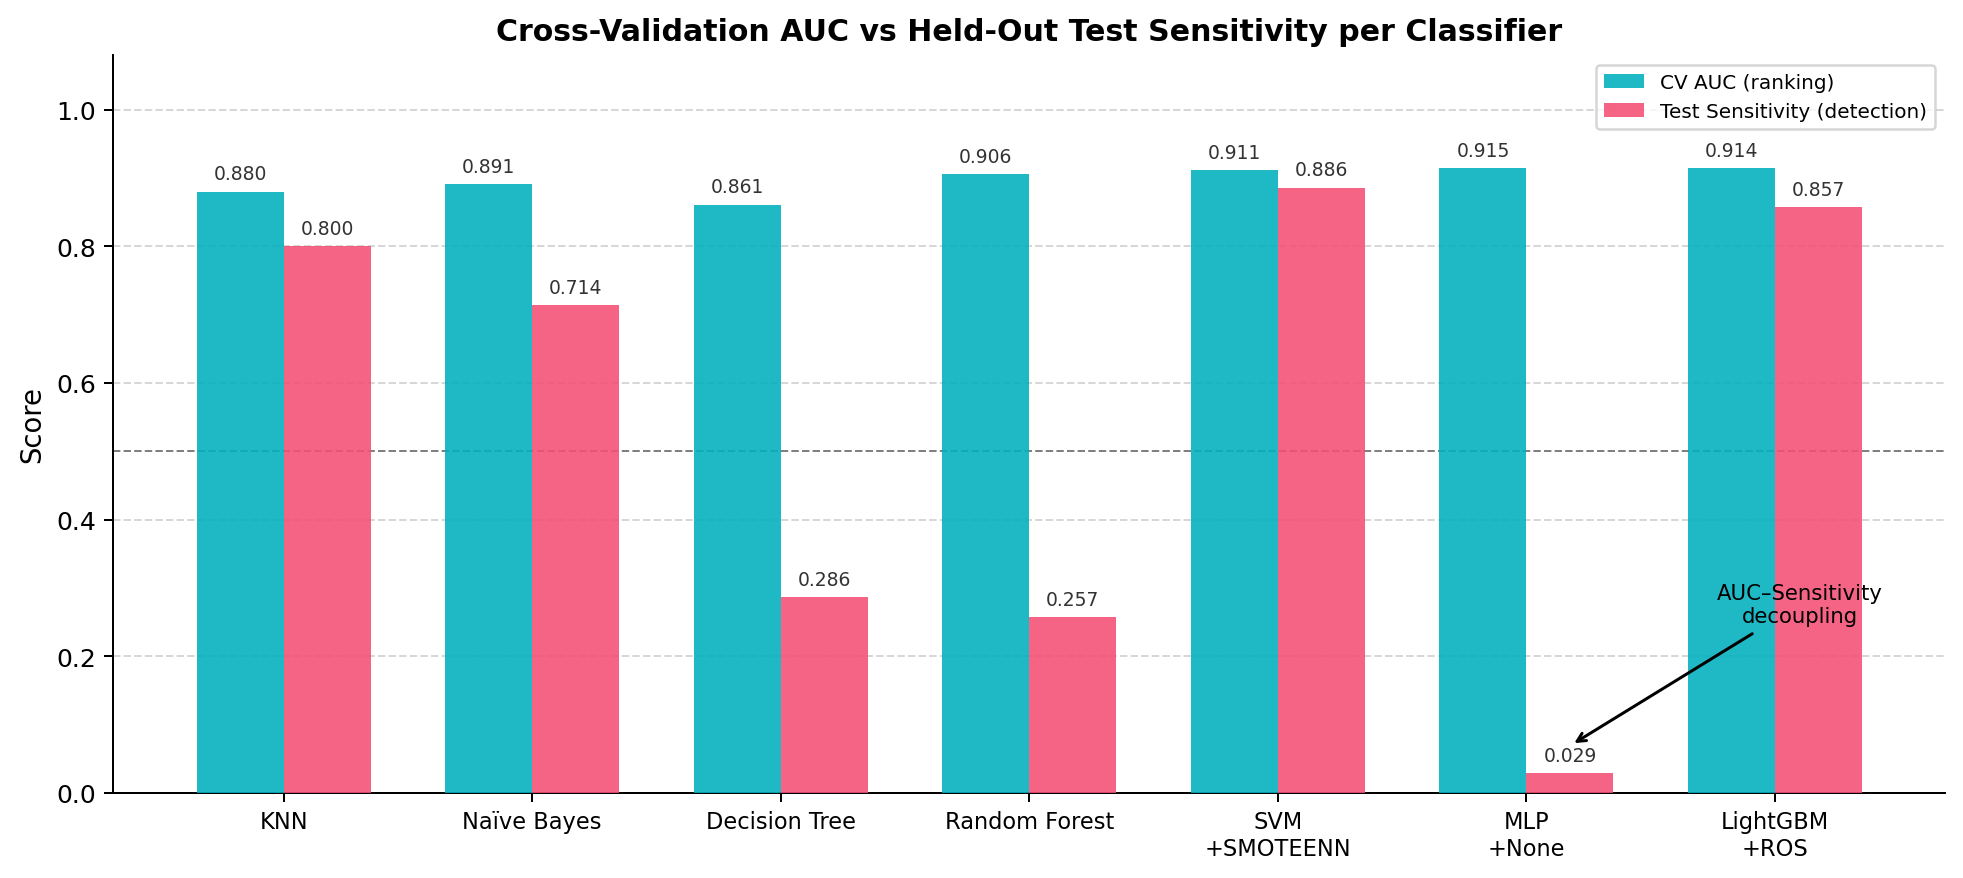
\includegraphics[width=0.95\linewidth]{images/figures/fig_auc_sensitivity_decoupling.png}
  \caption[CV AUC vs.\ test sensitivity: AUC--sensitivity decoupling]{Cross-validation AUC versus held-out test sensitivity for all seven classifiers. The MLP achieves the highest CV AUC (0.915) yet collapses to near-zero sensitivity (0.029), while LightGBM+ROS and SVM+SMOTEENN maintain sensitivity above 0.85 with competitive AUC values.}
  \label{fig:s2_decoupling}
\end{figure}

% ============================================================
\section{AUC--Sensitivity Decoupling}
\label{sec:s2r_decoupling}
% ============================================================

The MLP detected one Short Survivor out of 35.
Sensitivity is 0.029.
Balanced accuracy is 0.514 (essentially a coin flip).
A specificity of 1.000 is not a strength: it means the model labelled 34 of 35 Short Survivors as Standard Survival, as shown in Figure~\ref{fig:s2_cm}.
Yet its test AUC is 0.918, the third highest overall.

The name for this pattern is AUC--sensitivity decoupling.
AUC measures ranking ability---the probability that a positive instance receives a higher predicted score than a negative one---not the ability to classify correctly at a given threshold.
Under severe class imbalance (7.6:1), a model can learn to assign slightly higher probabilities to Short Survivors on average while still placing those probabilities well below the 0.5 decision boundary.
Cross-validation detects the ranking signal but does not expose the threshold mismatch; the held-out test makes it visible.

The precision-recall curves in Figure~\ref{fig:s2_pr} confirm this: despite an average precision of 0.669, the MLP's minority-class probabilities cluster below the decision threshold for nearly all patients, with only one crossing 0.5.

\begin{figure}[ht!]
  \centering
  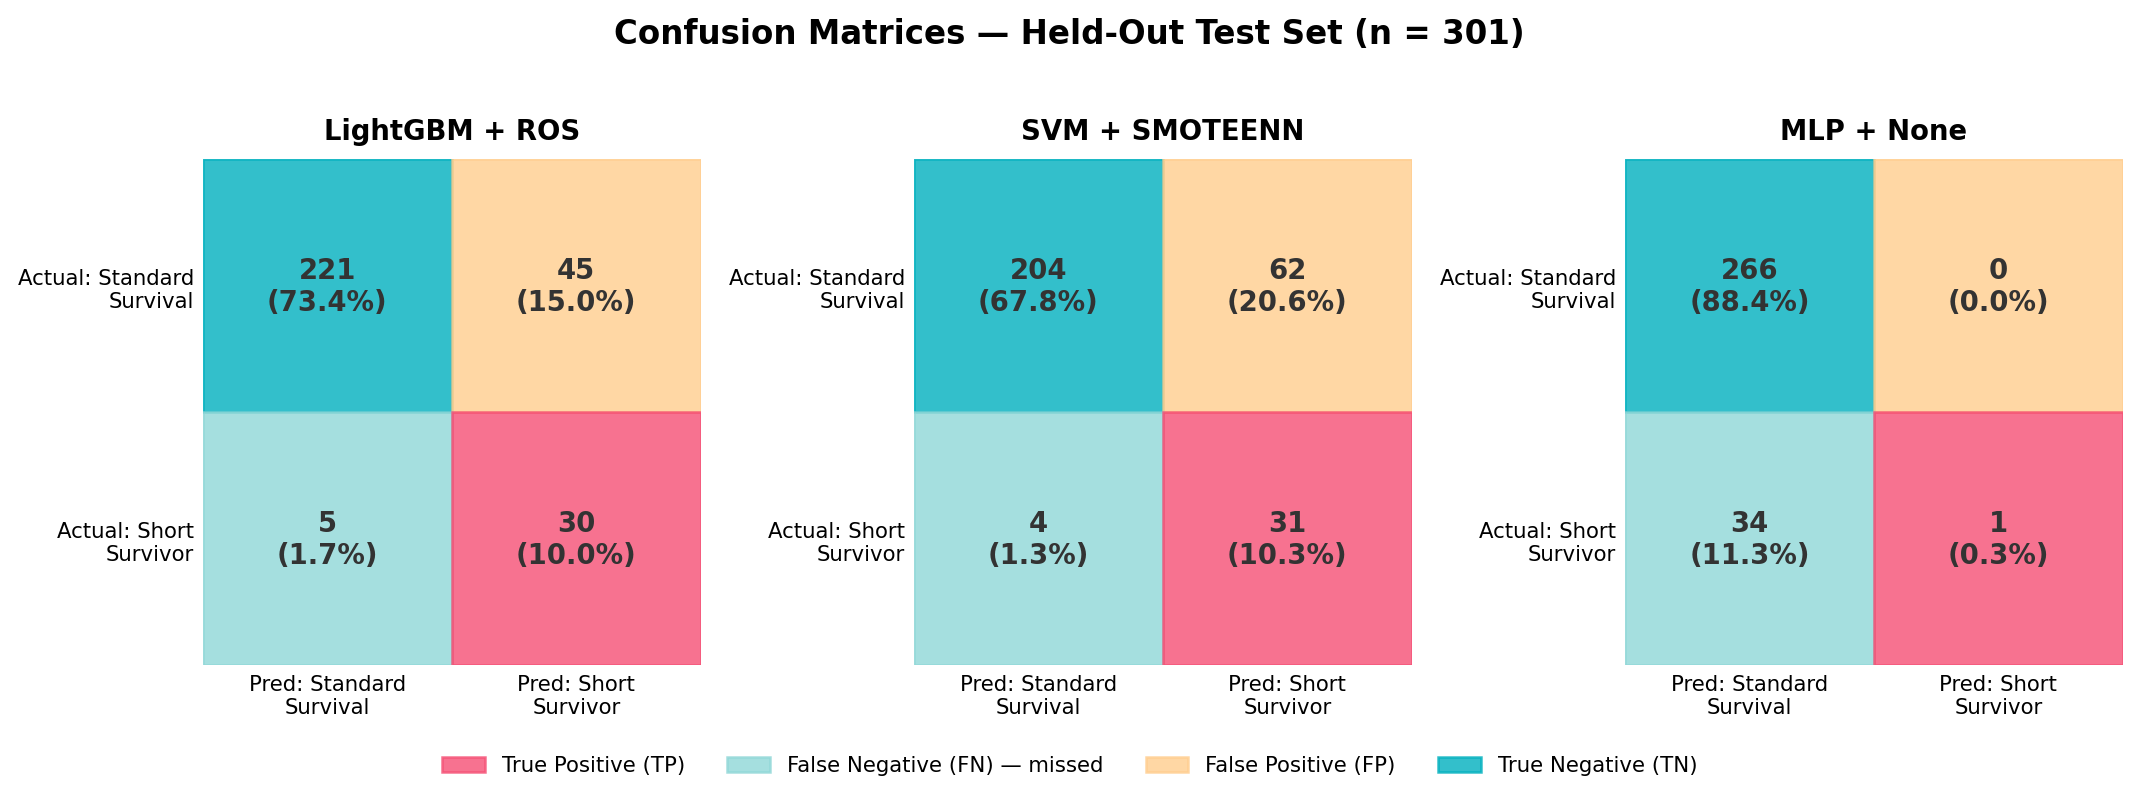
\includegraphics[width=0.97\linewidth]{images/figures/fig_confusion_matrices.png}
  \caption[Confusion matrices for three highlighted classifiers]{Confusion matrices on the held-out test set for the three classifiers highlighted in the text. LightGBM+ROS and SVM+SMOTEENN correctly identify the majority of Short Survivors (TP), whereas MLP+None effectively classifies all patients as Standard Survival (FN\,$= 34$).}
  \label{fig:s2_cm}
\end{figure}

\begin{figure}[ht!]
  \centering
  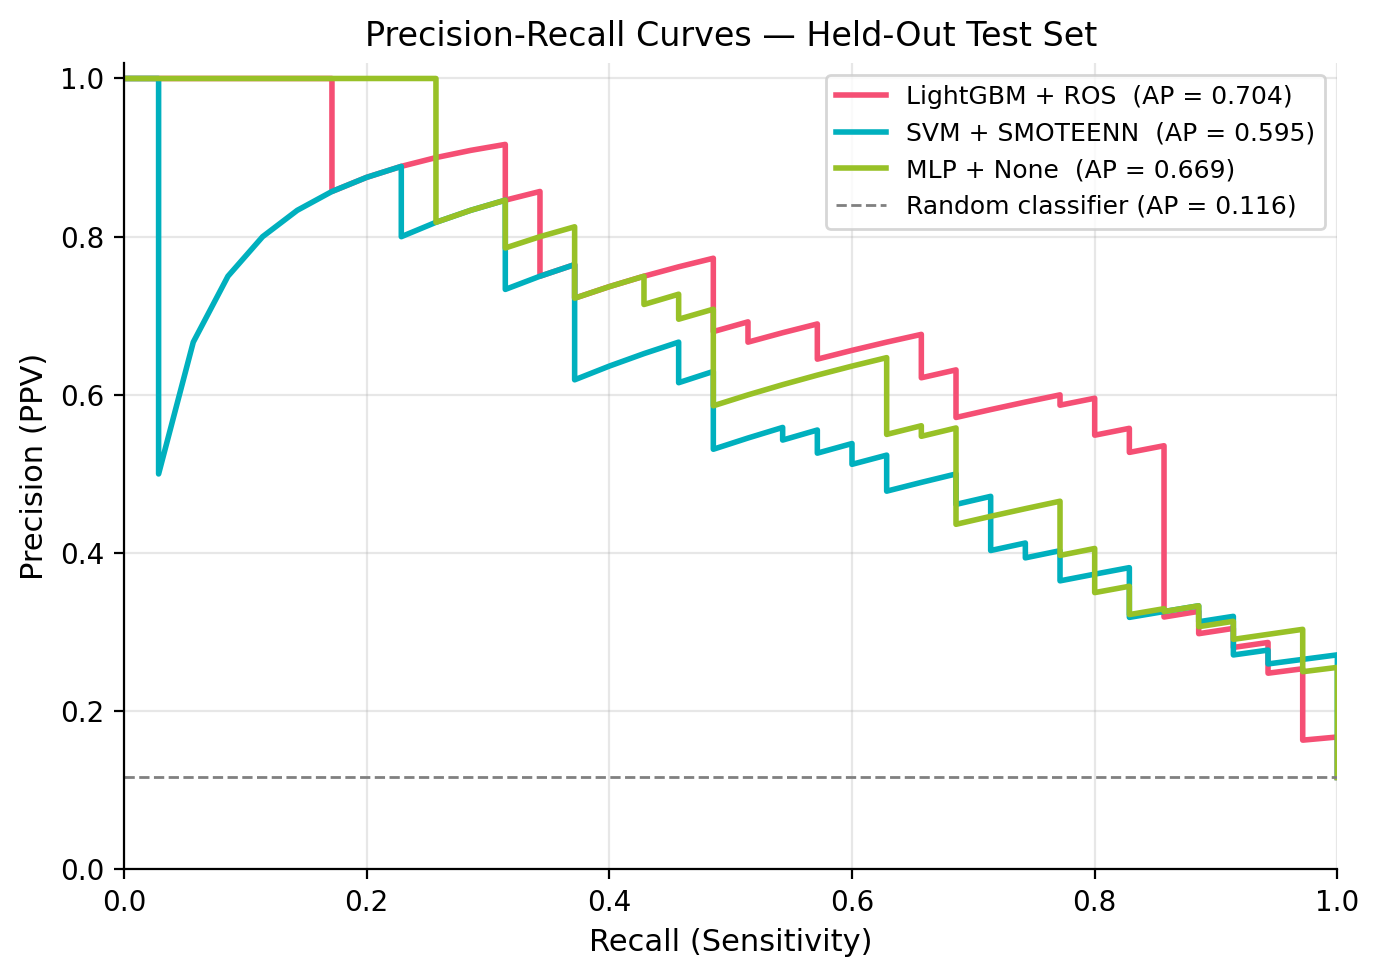
\includegraphics[width=0.95\linewidth]{images/figures/fig_pr_curves.png}
  \caption[Precision--Recall curves for three classifiers (Study II)]{Precision-recall curves on the held-out test set for the three highlighted classifiers. Despite a competitive average precision (LightGBM+ROS: 0.704, MLP: 0.669, SVM+SMOTEENN: 0.595), the MLP's minority-class probabilities cluster below the default threshold, collapsing to near-zero sensitivity at the operating point. The dashed line marks the random-classifier baseline (AP $\approx$ prevalence $\approx$ 0.116).}
  \label{fig:s2_pr}
\end{figure}

This finding reinforces the dissertation-wide argument (see also Section~\ref{sec:results_threshold_opt} for Study~I): ALS prognostic models must be evaluated not only by ranking metrics, but also by threshold behaviour and minority-class recall.
In a clinical setting, missing a Short Survivor means missing the window for timely palliative planning; high AUC without adequate sensitivity is clinically insufficient.

% ============================================================
\section{Decision Threshold Analysis}
\label{sec:s2r_threshold}
% ============================================================

The AUC--sensitivity gap motivates a systematic investigation of alternative decision thresholds.
Three thresholds were derived from out-of-fold (OOF) CV predictions for each classifier---ensuring no information from the held-out test set was used in their selection---and subsequently applied to the test set:
(i)~Youden's J~\cite{youden1950} (maximises sensitivity $+$ specificity $- 1$);
(ii)~sensitivity-constrained (highest threshold achieving $\geq 0.90$ sensitivity on OOF predictions);
and (iii)~F1-optimal (maximises minority-class F1 on OOF predictions).
Table~\ref{tab:s2_threshold} reports results for the two most instructive classifiers.

\begin{table}[ht!]
  \caption[Decision threshold analysis: MLP and LightGBM]{Test-set performance under three decision thresholds for MLP+None and LightGBM+ROS. Thresholds marked $\dagger$ were derived from out-of-fold CV predictions; the 0.50 row is the unmodified baseline. The sensitivity-constrained strategy ($\geq 0.90$) returned degenerate thresholds ($\approx\!0$) for both classifiers and is excluded. TP/FN counts are out of 35 Short Survivors.}
  \label{tab:s2_threshold}
  \resizebox{\linewidth}{!}{%
  \begin{tabular}{llcccccc}
    \toprule
    \textbf{Classifier} & \textbf{Threshold strategy} & \textbf{Threshold}
      & \textbf{Sensitivity} & \textbf{Specificity} & \textbf{Bal.\ Acc.}
      & \textbf{G-Mean} & \textbf{TP/FN} \\
    \midrule
    \multirow{3}{*}{MLP + None}
      & Default (0.50)       & 0.500 & 0.029 & 1.000 & 0.514 & 0.169 & 1\,/\,34 \\
      & Youden$^\dagger$     & 0.152 & 0.486 & 0.966 & 0.726 & 0.685 & 17\,/\,18 \\
      & F1-optimal$^\dagger$ & 0.239 & 0.371 & 0.981 & 0.676 & 0.604 & 13\,/\,22 \\
    \midrule
    \multirow{3}{*}{LightGBM + ROS}
      & Default (0.50)       & 0.500 & 0.857 & 0.831 & 0.844 & 0.844 & 30\,/\,5 \\
      & Youden$^\dagger$     & 0.404 & 0.857 & 0.778 & 0.818 & 0.817 & 30\,/\,5 \\
      & F1-optimal$^\dagger$ & 0.656 & 0.800 & 0.925 & 0.862 & 0.860 & 28\,/\,7 \\
    \bottomrule
  \end{tabular}%
  }
\end{table}

Lowering the MLP threshold from 0.500 to the Youden value (0.152) raises sensitivity from 0.029 to 0.486---16 additional Short Survivors correctly identified---while retaining high specificity (0.966).
The F1-optimal threshold (0.239) yields a more conservative recovery (sensitivity 0.371, specificity 0.981).
Even under optimal threshold selection, however, the MLP's best sensitivity (0.486) remains well below that of LightGBM+ROS at the default boundary (0.857), confirming that the AUC--sensitivity decoupling is structural rather than a threshold artefact.

For LightGBM+ROS, the Youden threshold (0.404) detects the same number of Short Survivors as the default (30 of 35), with a modest specificity trade-off.
The F1-optimal threshold (0.656) shifts the balance toward specificity (0.925), missing two additional patients, and yields the highest G-Mean across all configurations in this table (0.860).

The sensitivity-constrained analysis (targeting $\geq 0.90$ sensitivity) produced degenerate thresholds ($\approx\!0$) for both classifiers, meaning no threshold achieves 90\% sensitivity with meaningful specificity under the current feature set.
This signals a dataset-level ceiling on Short Survivor recall that neither resampling nor threshold selection can overcome without additional discriminative features.

% ============================================================
\section{BalancedBagging Replication and Statistical Validation}
\label{sec:s2r_bagging}
% ============================================================

Table~\ref{tab:s2_bonferroni} reports mean balanced accuracy for each classifier under single-model and BalancedBagging configurations, along with the statistical comparison.

\begin{table}[ht!]
  \centering
  \caption[BalancedBagging vs.\ single classifier (CV balanced accuracy)]{Cross-validation balanced accuracy under single-model and BalancedBagging configurations, with per-fold Wilcoxon signed-rank tests (Bonferroni-corrected for 7 comparisons). $^{***}p \leq 0.001$; $^{**}p \leq 0.01$; n.s.\ = not significant.}
  \label{tab:s2_bonferroni}
  \resizebox{\linewidth}{!}{%
  \begin{tabular}{lcccc}
    \toprule
    \textbf{Classifier} & \textbf{Single-Model} & \textbf{BalancedBagging}
      & \textbf{$\Delta$} & \textbf{$p$ (Bonf.)} \\
    \midrule
    KNN           & 0.566 & 0.788 & $+$0.221 & $<0.001^{***}$ \\
    Naïve Bayes   & 0.797 & 0.809 & $+$0.012 & $>$0.999 n.s.  \\
    Decision Tree & 0.653 & 0.777 & $+$0.125 & $0.001^{**}$   \\
    Random Forest & 0.629 & 0.814 & $+$0.185 & $<0.001^{***}$ \\
    SVM           & 0.500 & 0.793 & $+$0.293 & $<0.001^{***}$ \\
    MLP           & 0.698 & 0.832 & $+$0.134 & $<0.001^{***}$ \\
    LightGBM      & 0.692 & 0.820 & $+$0.128 & $<0.001^{***}$ \\
    \bottomrule
  \end{tabular}%
  }
\end{table}

Six of seven classifiers exhibit a statistically significant improvement in balanced accuracy under BalancedBagging ($p \leq 0.01$ after Bonferroni correction).
The sole exception is Naïve Bayes ($p > 0.999$, n.s.): its generative modelling of class-conditional densities makes it relatively insensitive to training class proportions, and its single-model balanced accuracy (0.797) already approaches its ensemble counterpart (0.809).

The SVM shows the largest absolute gain ($\Delta = +0.293$), crossing from a balanced accuracy of 0.500 to 0.793 once internal balancing is applied within each bootstrap sample.
The MLP achieves the highest ensemble balanced accuracy (0.832), consistent with the reference study's findings.
LightGBM also improves significantly under BalancedBagging ($\Delta = +0.128$, $p < 0.001$), demonstrating that the ensemble strategy generalises beyond the six classifiers of the original work.

% ============================================================
\section{Comparison with the Reference Study}
\label{sec:s2r_comparison}
% ============================================================

Table~\ref{tab:s2_comparison} summarises the methodological and performance differences between the reference study and Study~II.

\begin{table}[ht!]
  \centering
  \caption[Comparison with Papaiz et al.\ (2024)]{Direct comparison between Papaiz et al.~\cite{Papaiz2024} and Study~II. \textsuperscript{a}Best ensemble balanced accuracy reported under repeated CV. \textsuperscript{b}Not reported in the reference study.}
  \label{tab:s2_comparison}
  \resizebox{\linewidth}{!}{%
  \begin{tabular}{lcc}
    \toprule
    \textbf{Aspect} & \textbf{Papaiz et al.~\cite{Papaiz2024}} & \textbf{Study~II} \\
    \midrule
    Patients                                   & 1,967              & 1,502              \\
    Classifiers evaluated                      & 6                  & 7 (+LightGBM)      \\
    Imbalance strategies                       & BalancedBagging    & 10 strategies + BB \\
    Hyperparameter optimisation                & Grid search        & Bayesian (Optuna)  \\
    Best CV Bal.\ Acc.\ (MLP+BB)\textsuperscript{a} & $\approx$0.84 & 0.832 \\
    Held-out test evaluation                   & No\textsuperscript{b} & Yes             \\
    Best test AUC                              & ---\textsuperscript{b} & 0.923 (LightGBM+ROS) \\
    Best test Sensitivity                      & ---\textsuperscript{b} & 0.857 (LightGBM+ROS) \\
    Explainability (SHAP)                      & Yes (6 classifiers) & Yes (TreeSHAP + KernelSHAP) \\
    \bottomrule
  \end{tabular}%
  }
\end{table}

The CV balanced accuracy for MLP+BalancedBagging (0.832) closely matches the reference figure ($\approx$0.84) on a smaller, more imbalanced cohort.
The minor gap reflects the smaller cohort (1,502 versus 1,967 patients), the higher imbalance ratio (7.6 versus 6.9), and minor differences in the PRO-ACT extract available.
The per-classifier pattern of gains mirrors the original paper across all seven classifiers, suggesting its conclusions hold across different PRO-ACT extracts.

Three additions matter beyond the replication.
Bayesian optimisation finds hyperparameter configurations---particularly the MLP's high L2 penalty---that grid search would rarely reach.
LightGBM adds a gradient-boosted option the original study did not test, and it proves to be the most balanced performer on the held-out set.
The held-out test reveals that MLP's cross-validation lead does not hold under unseen data, a finding invisible in the reference study's CV-only design.

% ============================================================
\section{SHAP-Based Interpretation}
\label{sec:s2r_shap}
% ============================================================

Figure~\ref{fig:s2_shap} shows the TreeSHAP output for LightGBM+ROS on the held-out test set, with features ranked by mean absolute SHAP value.

\begin{figure}[ht!]
  \centering
  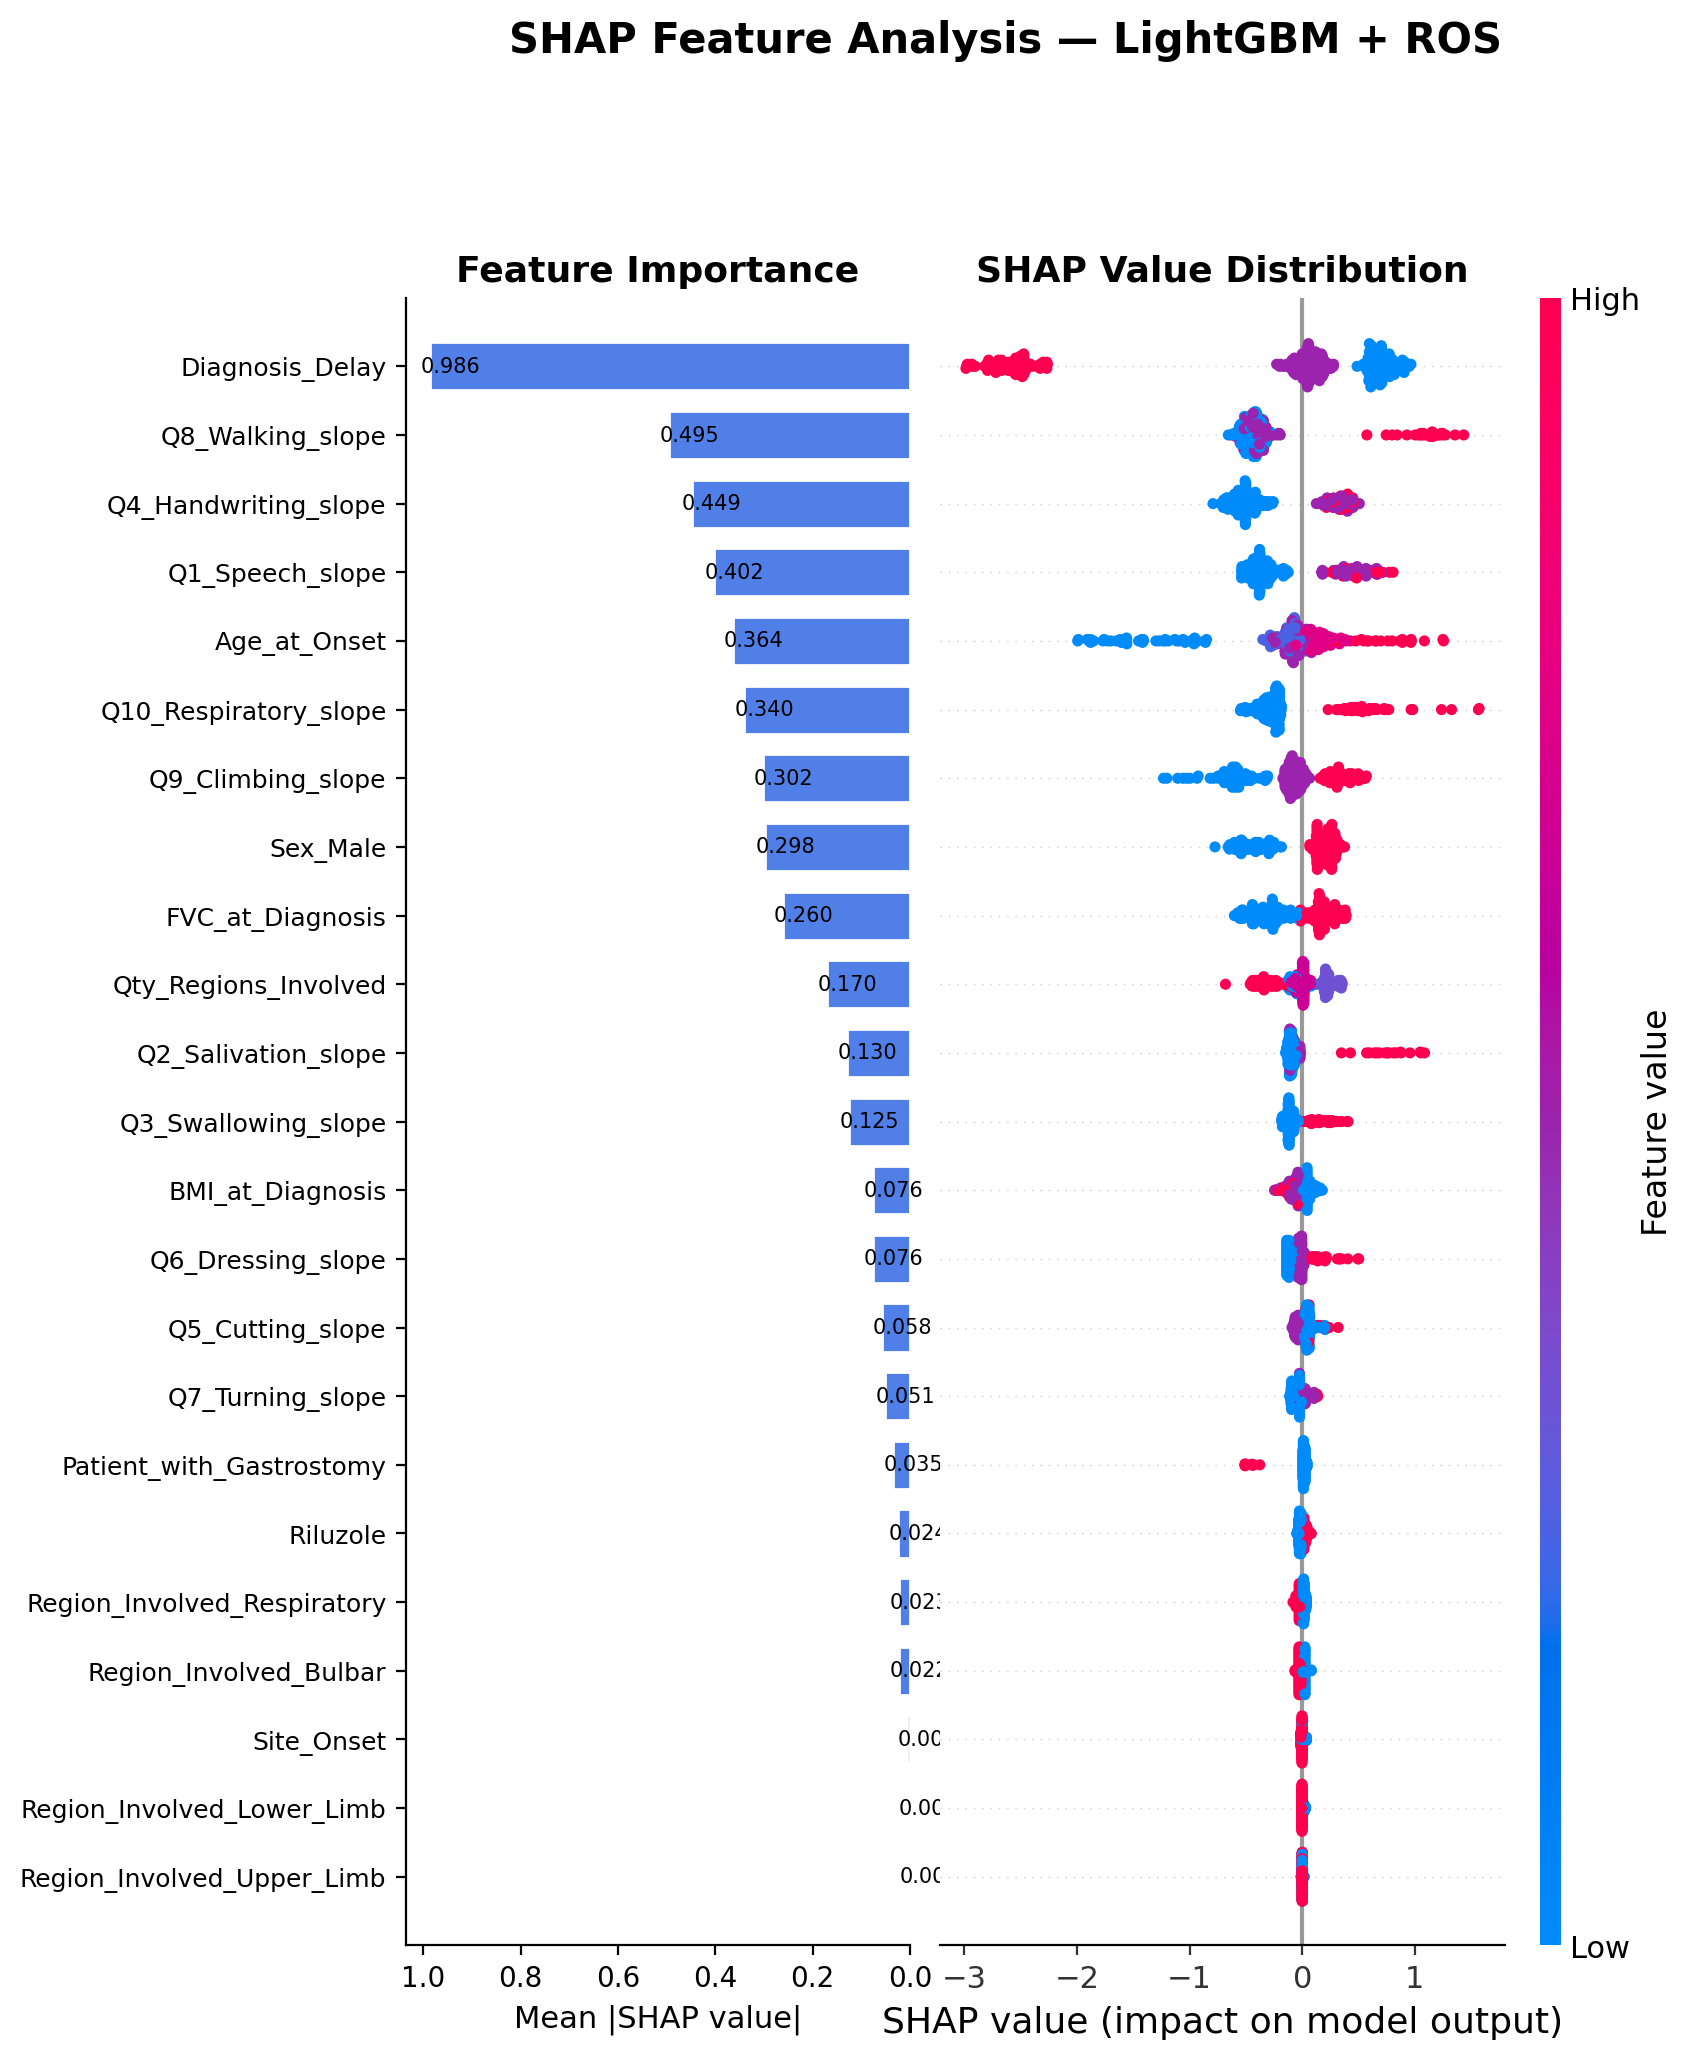
\includegraphics[width=0.95\linewidth]{images/figures/step7_lightgbm_fig3_combined.png}
  \caption[SHAP feature importance: LightGBM+ROS (Study II)]{SHAP feature importance for LightGBM+ROS (held-out test set). \textit{Left:} global bar chart of mean $|\text{SHAP}|$ values. \textit{Right:} beeswarm plot showing per-instance SHAP contributions, coloured by feature value (red = high, blue = low).}
  \label{fig:s2_shap}
\end{figure}

\texttt{Diagnosis\_Delay} is the dominant predictor (mean $|\text{SHAP}| = 0.986$), more than double the next-ranked feature.
Long delays associate with Standard Survival; short delays signal rapid pre-diagnosis progression and Short Survivor risk, consistent with clinical observations~\cite{Feldman2022}.

ALSFRS-R slopes fill ranks two through four and six: Q8 (walking), Q4 (handwriting), Q1 (speech), Q10 (respiratory).
Age at onset is fifth ($|\text{SHAP}| = 0.364$); older patients tend to progress faster.
FVC at diagnosis ranks ninth ($|\text{SHAP}| = 0.260$), adding a respiratory dimension.
This ranking is consistent with the reference study's SHAP output~\cite{Papaiz2024}.

The parallel KernelSHAP analysis of the MLP found the same top feature and a broadly similar slope ranking, though with smaller absolute attributions, expected given the more diffuse weight structure of neural networks.

Figure~\ref{fig:s2_featbars} shows how \texttt{Diagnosis\_Delay} and Q8 separate the two groups at the population level.

\begin{figure}[ht!]
  \centering
  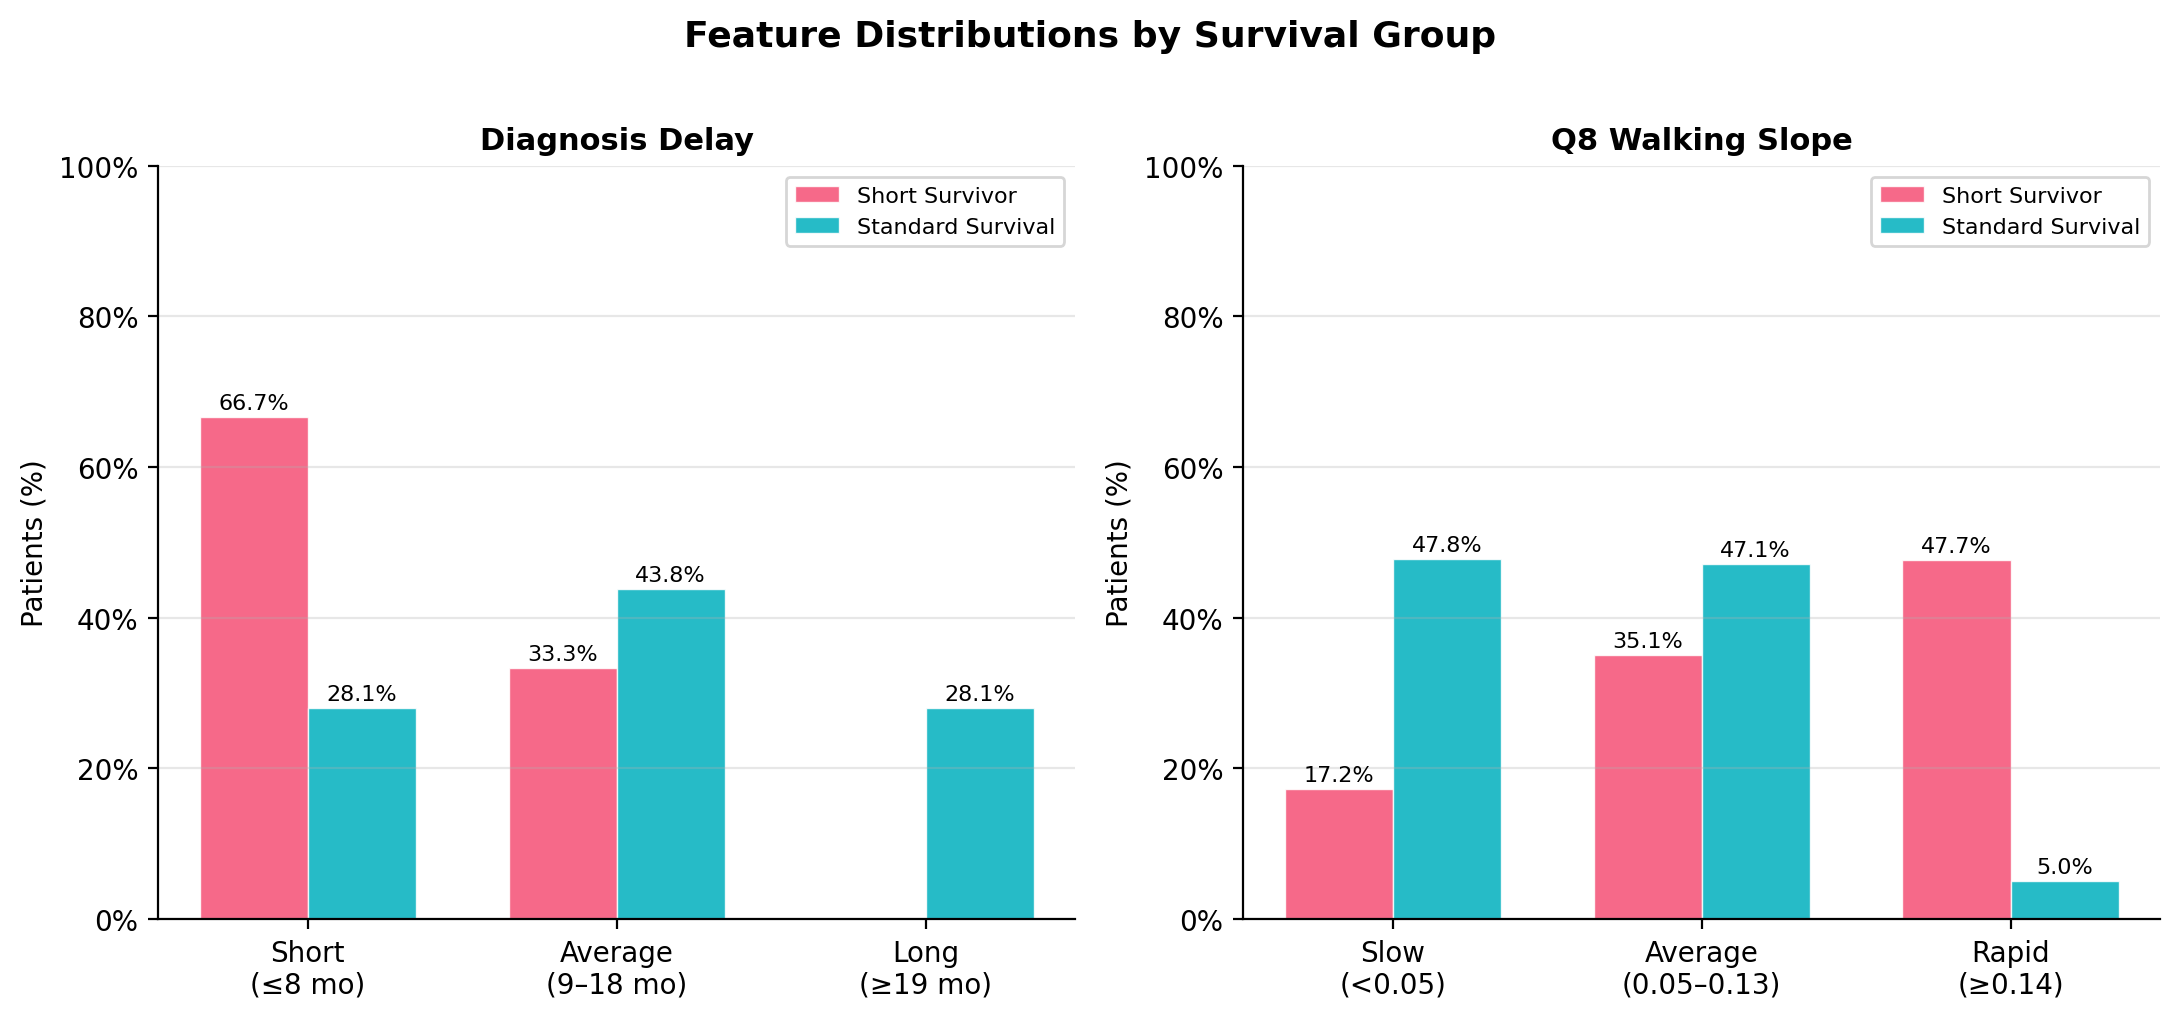
\includegraphics[width=0.97\linewidth]{images/figures/fig_feature_bars.png}
  \caption[Feature distributions by survival group]{Distribution of \texttt{Diagnosis\_Delay} (left) and \texttt{Q8\_Walking\_slope} (right) by survival group across the full dataset. Short Survivors are disproportionately concentrated in the short-delay and rapid-slope categories, consistent with their SHAP importance rankings.}
  \label{fig:s2_featbars}
\end{figure}

% ============================================================
\section{Limitations}
\label{sec:s2r_limitations}
% ============================================================

Several limitations apply to the results of Study~II.

\begin{enumerate}
  \item \textbf{Smaller cohort.} The 1,502-patient cohort is 23.6\% smaller than Papaiz et al.'s 1,967, primarily due to FVC missingness in the publicly available PRO-ACT extract (62.3\% missing post-filters). Patients with complete FVC records may differ systematically from those without, introducing potential selection bias.
  \item \textbf{Internal test set only.} Train and test sets are drawn from the same PRO-ACT extract. No external validation was performed. Results may not generalise to other clinical populations, different ALS registries, or healthcare systems with different referral patterns.
  \item \textbf{Small minority-class test set.} Only 35 Short Survivors appear in the test set. One patient equals 2.86 percentage points of sensitivity, making point estimates highly sensitive to individual predictions. Bootstrap confidence intervals confirm wide uncertainty (e.g., LightGBM+ROS recall CI: [0.724,\,0.967]).
  \item \textbf{Post-diagnosis ALSFRS-R slope risk.} Where no pre-diagnosis assessment was available, the nearest visit was used. For a subset of patients, this introduces limited post-diagnosis information into the predictor set, a constraint inherited from the reference study's design.
  \item \textbf{Feature set inherited from the reference study.} The 23 ordinal/binary features were chosen to match Papaiz et al.\ for direct comparison, not necessarily to maximise predictive performance. Alternative or richer feature representations may yield better discrimination.
  \item \textbf{Survival target depends on censoring assumptions.} Subjects alive at last observation with follow-up $> 24$ months are classified as Standard Survival, which may include patients who die shortly after. The 24-month threshold follows the reference study exactly.
\end{enumerate}

% ============================================================
\section{Summary}
\label{sec:s2r_summary}
% ============================================================

Study~II confirms the central finding of Papaiz et al.~\cite{Papaiz2024}: BalancedBagging significantly improves balanced accuracy in six of seven classifiers under severe ALS survival class imbalance, with the MLP achieving the highest ensemble balanced accuracy (0.832 versus the reference's $\approx$0.84).

Beyond replication, LightGBM with Random Oversampling emerges as the most effective single model, achieving AUC 0.923 and sensitivity 0.857 on the held-out test set---outperforming all six classifiers evaluated in the reference study.

The most consequential finding is the AUC--sensitivity decoupling: the MLP achieves the second-highest test AUC (0.918) while detecting only 1 of 35 Short Survivors at the default threshold (sensitivity 0.029).
Threshold optimisation using Youden's J raises MLP sensitivity to 0.486, but this remains well below LightGBM+ROS at its default threshold, confirming the decoupling is structural.

SHAP analysis consistently identifies \texttt{Diagnosis\_Delay} as the dominant predictor (mean $|\text{SHAP}| = 0.986$), followed by ALSFRS-R functional decline slopes.
These findings are robust across both TreeSHAP (LightGBM) and KernelSHAP (MLP), and are consistent with the reference study's interpretations.

Taken together, Study~II demonstrates that imbalance-aware learning can improve ALS survival prognosis, while also showing that high ROC-AUC can mask clinically unacceptable minority-class recall.
These findings reinforce the dissertation's broader argument: ALS prognostic modelling must be evaluated through threshold behaviour, minority-class sensitivity, and interpretability, not ranking metrics alone.

